% This is samplepaper.tex, a sample chapter demonstrating the
% LLNCS macro package for Springer Computer Science proceedings;
% Version 2.21 of 2022/01/12
%
\documentclass[runningheads]{llncs}
%
\usepackage[T1]{fontenc}
% T1 fonts will be used to generate the final print and online PDFs,
% so please use T1 fonts in your manuscript whenever possible.
% Other font encondings may result in incorrect characters.


% tightlist command for lists without linebreak
\providecommand{\tightlist}{%
  \setlength{\itemsep}{0pt}\setlength{\parskip}{0pt}}




\usepackage{graphicx}
% Used for displaying a sample figure. If possible, figure files should
% be included in EPS format.
%
% If you use the hyperref package, please uncomment the following two lines
% to display URLs in blue roman font according to Springer's eBook style:
\usepackage{hyperref}
\usepackage{color}
\renewcommand\UrlFont{\color{blue}\rmfamily}


\begin{document}


\title{Práctica en R-Studio\thanks{INTA Eugenio Bustos}}
%
\titlerunning{Práctica en R-Studio}
% If the paper title is too long for the running head, you can set
% an abbreviated paper title here
%
\author{Ian Johnson\inst{1}\orcidID{0009-0001-2786-9385} \and Carolina
Fernández\inst{1}\orcidID{0009-0004-4219-1041} \and Julián
Hidalgo\inst{1}\orcidID{0009-0002-0617-6800}}


\authorrunning{Grupo Los Ignorantes}
% First names are abbreviated in the running head.
% If there are more than two authors, 'et al.' is used.
%

\institute{Grupo Los Ignorantes}

\maketitle              % typeset the header of the contribution
%
\begin{abstract}
En este documento se agregan imágenes, ecuaciones y tablas usando el
R-Markdown.

\keywords{Imágenes \and Ecuaciones \and Tablas \and R-Studio}

\end{abstract}

\hypertarget{primera-secciuxf3n}{%
\section{Primera sección}\label{primera-secciuxf3n}}

\hypertarget{movimiento-armuxf3nico-simple}{%
\subsection{Movimiento Armónico
Simple}\label{movimiento-armuxf3nico-simple}}

La ecuación del movimiento armónico simple es:

\begin{equation}
y = A cos(\omega t + \phi)
\end{equation}

\begin{figure}
\centering
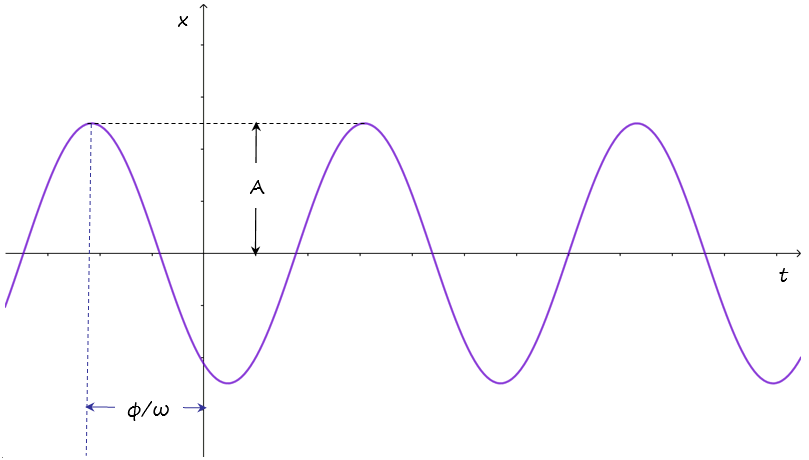
\includegraphics[width=3.125in,height=2.34375in]{MAS.png}
\caption{Movimiento Armónico Simple}
\end{figure}

\hypertarget{ecuaciuxf3n-de-bernoulli}{%
\subsection{Ecuación de Bernoulli}\label{ecuaciuxf3n-de-bernoulli}}

La ecuación de Bernoulli es:

\begin{equation}
P_1 + \frac{1}{2} \rho (v_1)^2 + \rho g h_1 = P_2 + \frac{1}{2} \rho (v_2)^2 + \rho g h_2 
\end{equation}

\begin{figure}
\centering
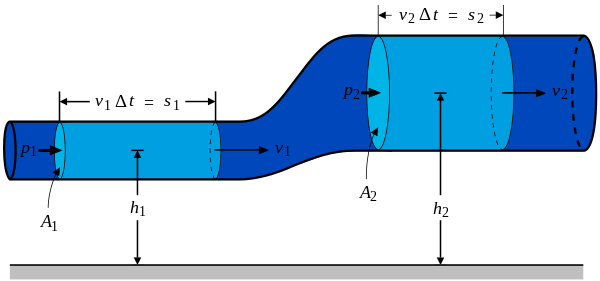
\includegraphics[width=3.125in,height=1.5625in]{BernoullisLawDerivationDiagram.svg.png}
\caption{Bernoulli}
\end{figure}

\hypertarget{pbi-per-cuxe1pita-de-argentina}{%
\subsection{PBI per cápita de
Argentina}\label{pbi-per-cuxe1pita-de-argentina}}

La tabla \ref{tab:table} muestra la evolución del PBI per cápita de
Argentina durante el período entre 2011 y 2021

\begin{table}

\caption{\label{tab:table}PBI per cápita de Argentina entre 2011 y 2021}
\centering
\begin{tabular}[t]{r|r}
\hline
Año & PBI\\
\hline
2021 & 10.625\\
\hline
2020 & 8.574\\
\hline
2019 & 10.054\\
\hline
2018 & 11.786\\
\hline
2017 & 14.618\\
\hline
2016 & 12.773\\
\hline
\end{tabular}
\end{table}

%
% ---- Bibliography ----



\end{document}
